\section{Legge dei punti coniugati e ingrandimento}
L'ultima parte dell'esperienza riguarda l'ottica delle lenti sottili. Una lente sottile doppio-convessa in plastica trasparente ha un'indice di rifrazione maggiore dell'aria. Pertanto, la luce che attraversa una lente subirà, per la legge di Snell, due rifrazioni consecutive. Un fascio di raggi paralleli incidenti in una lente viene concentrato in un punto F detto punto focale o fuoco. La distanza tra il punto focale e l'asse della lente sottile viene detta distanza focale e indicata con $f$. Si indicano invece con $p$ e $q$ rispettivamente la distanza oggetto-lente e la distanza lente-immagine.
Queste distanze sono legate tra loro dalla legge dei punti coniugati\\
\begin{equation}
    \frac{1}{f} = \frac{1}{p} + \frac{1}{q}
    \label{eq:punti-coniugati}
\end{equation}
Un'immagine è a fuoco quando i raggi luminosi che attraversano la lente colpiscono uno schermo a distanza focale, ovvero quando i raggi si intersecano nel punto focale. Quando l'immagine è a fuoco è nitida e generalmente ingrandita. Si definisce ingrandimento trasversale\\ 
\begin{equation}
    M=\frac{L_{immagine}}{L_{oggetto}}
    \label{eq:ingrandimento-sperimentale}
\end{equation}
e per geometria 
\begin{equation}
    M=\frac{q}{p}
    \label{eq:ingrandimento-teorico}
\end{equation}
Dalla legge dei punti coniugati si può inoltre ricavare una distanza minima tra schermo e sorgente oltre la quale non è più possibile mettere a fuoco l'immagine. Sia $D=p+q$ la distanza: posso sostituire $q=D-p$ nella \eqref{eq:punti-coniugati} e otttenere $$\frac{1}{f}=\frac{D}{(D-p)\;p}$$
Sviluppando i calcoli si ottiene un'equazione di secondo grado nell'incognita $p$, che ha soluzioni reali solo per $\Delta>0$, ovvero per $D \geq 4f$, da cui $D_{min}=4f$.

Questa fase dell'esperienza ha lo scopo di verificare la legge dei punti coniugati misurando la distanza focale di due lenti a focale diversa con un banco ottico e di confrontare l'ingrandimento sperimentale con quello previsto. Per fare ciò un'immagine millimetrata a forma di croce viene proiettata attraverso la lente su uno schermo posto a distanze dalla sorgente variabili. Per ciascuna distanza si misurano due valori distinti di  $p$ e $q$, data la natura simmetrica della \eqref{eq:punti-coniugati}, e la lunghezza del braccio graduato. Si interpolano linearmente $\frac{1}{p}$ e $\frac{1}{q}$ e si ricava la distanza focale dall'inverso del parametro corrispondente all'intercetta. Infine si calcola dalla relazione \eqref{eq:ingrandimento-sperimentale} l'ingrandimento sperimentale e lo si confronta con quello teorico previsto dalla relazione \eqref{eq:ingrandimento-teorico}. Si 

\subsection{Lente con focale di \qty{250}{mm}}
La prima lente utilizzata per questa fase dell'esperimento ha focale di \qty{250}{mm}. Si raccolgono in una tabella di seguito le misure di $p$ e $q$ a distanze crescenti.\\
\begin{table}[htbp]
\begin{center}
\setlength{\tabcolsep}{8pt} 
\renewcommand{\arraystretch}{1.2} 
\small 

\begin{tabular}{ccccc}
\toprule
% Impostiamo multirow su 3 righe fittizie per compensare l'altezza del testo a sinistra
\multirow{2}{*}{\begin{tabular}[c]{@{}c@{}}\textbf{Distanza}\\\textbf{(\unit{mm})}\end{tabular}} & \multicolumn{2}{c}{\textbf{Misura 1}} & \multicolumn{2}{c}{\textbf{Misura 2}} \\
\cmidrule(r){2-3} \cmidrule(l){4-5}
 & \textbf{$p$ (\unit{mm})} & \textbf{$q$ (\unit{mm})} & \textbf{$p$ (\unit{mm})} & \textbf{$q$ (\unit{mm})} \\
\midrule
1100 & 390 & 710  & 720  & 380 \\
1200 & 355 & 845  & 850  & 350 \\
1300 & 340 & 960  & 968  & 332 \\
1400 & 329 & 1071 & 1074 & 326 \\
1500 & 319 & 1181 & 1186 & 314 \\
\bottomrule
\end{tabular}
\vspace{0.3cm}
\caption{Valori di $p$ e $q$ per una lente di focale \qty{250}{mm} a distanze variabili.}
\label{tab:distanze-focali-1}
\end{center}
\end{table}

Alle misure di $p$ e $q$ è stata associata un'incertezza di \qty{1}{cm} dovuta alla difficoltà di trovare visivamente il punto di fuoco dell'immagine. 
Successivamente sono stati interpolati linearmente con due parametri liberi a e b $\frac{1}{p}$ e $\frac{1}{q}$. Dall'interpolazione, di cui si riporta il grafico qui sotto, si ricava un coefficiente angolare $b = (-1.02 \pm 0.02)$, compatibile con $-1$, 
come previsto da \eqref{eq:punti-coniugati}, e l'intercetta $a = (4.04 \pm 0.05) \times 10^{-3}$, 
da cui si ricava $f = \qty{247.5 \pm 3.1}{mm}$.\\

\begin{figure}[H]
    \centering
    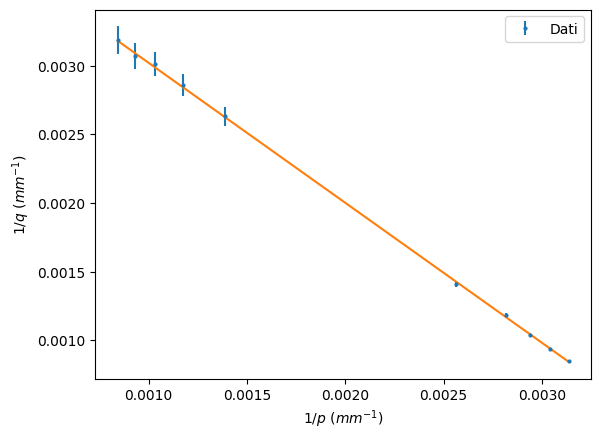
\includegraphics[width=0.56\textwidth]{immagini/250mm.png}
    \caption{Interpolazione lineare tra $\frac{1}{p}$ e $\frac{1}{q}$}
    \label{fig:2}
\end{figure}

Il test di adattamento del $\chi^2$ indica un adattamento del modello lineare del 93.2\%.
Il t-test restituisce t=0.80, associato a una compatibilità del 59,9\% con la distanza focale indicata sulla lente.\\
Si riportano quindi in un'ulteriore tabella gli ingrandimenti trasversali sperimentali misurati e i valori teorici calcolati tramite la relazione \eqref{eq:ingrandimento-teorico}. Per l'ingrandimento sperimentale si considera un'incertezza di \qty{1}{mm}, corrispondente alla precisione dello strumento di misura, sul valore di $L_{misurato}$.  È stata assunta la stessa incertezza anche sul valore di $L_{oggetto}$, benché fosse dato pari a \qty{40}{mm}, poiché la forma della figura non rendeva possibile verificare tale valore.
Per quanto riguarda $p$ e $q$, gli errori considerati sono gli stessi del punto precedente.

\begin{table}[htbp]
\centering
\begin{tabular}{c|cc|cc}
\hline
\hline
\textbf{Distanza} & \multicolumn{2}{c|}{\textbf{Misura 1}} & \multicolumn{2}{c}{\textbf{Misura 2}} \\
(\unit{mm}) & $M_{\text{sperimentale}}$ & $M_{\text{teorico}}$ & $M_{\text{sperimentale}}$ & $M_{\text{teorico}}$ \\
\hline
1100 & \qty{1.925 \pm 0.025}{} & \qty{1.821 \pm 0.053}{} & \qty{0.550 \pm 0.025}{} & \qty{0.528 \pm 0.016}{} \\
1200 & \qty{2.500 \pm 0.025}{} & \qty{2.380 \pm 0.073}{} & \qty{0.450 \pm 0.025}{} & \qty{0.412 \pm 0.013}{} \\
1300 & \qty{2.975 \pm 0.025}{} & \qty{2.824 \pm 0.088}{} & \qty{0.375 \pm 0.025}{} & \qty{0.343 \pm 0.011}{} \\
1400 & \qty{3.425 \pm 0.025}{} & \qty{3.255 \pm 0.104}{} & \qty{0.325 \pm 0.025}{} & \qty{0.304 \pm 0.010}{} \\
1500 & \qty{3.875 \pm 0.025}{} & \qty{3.702 \pm 0.120}{} & \qty{0.300 \pm 0.025}{} & \qty{0.265 \pm 0.009}{} \\
\hline
\hline
\end{tabular}
\caption{Confronto tra ingrandimento sperimentale e teorico al variare della distanza.}
\label{tab:confronto_ingrandimenti}
\end{table}

La compatibilità tra i valori sperimentali e quelli teorici è stata verificata tramite il t-test di Student; per ogni coppia di dati si è ottenuto t<2, confermando la compatibilità statistica delle misure.
È stata infine misurata la distanza minima sperimentale tra schermo e sorgente, pari a \qty{999 \pm 5}{mm}, compatibile con quella teorica, che per la lente usata corrisponde a \qty{1000}{mm}.

\subsection{Lente con focale di \qty{100}{mm}}
Le misure sono state ripetute in maniera analoga per la lente con focale pari a \qty{100}{mm}, considerando le stesse incertezze su ogni misura effettuata. Si riportano dunque i risultati ottenuti in maniera più concisa.
Sono state raccolte le misure di $p$ e $q$ per quattro distanze diverse, riportate di seguito:

\begin{table}[htbp]
\begin{center}
\setlength{\tabcolsep}{8pt} 
\renewcommand{\arraystretch}{1.2} 
\small 

\begin{tabular}{ccccc}
\toprule
% Impostiamo multirow su 2 righe fittizie per compensare l'altezza del testo a sinistra
\multirow{2}{*}{\begin{tabular}[c]{@{}c@{}}\textbf{Distanza}\\\textbf{(\unit{mm})}\end{tabular}} & \multicolumn{2}{c}{\textbf{Misura 1}} & \multicolumn{2}{c}{\textbf{Misura 2}} \\
\cmidrule(r){2-3} \cmidrule(l){4-5}
 & \textbf{$p$ (\unit{mm})} & \textbf{$q$ (\unit{mm})} & \textbf{$p$ (\unit{mm})} & \textbf{$q$ (\unit{mm})} \\
\midrule
600 & 139,0 & 461 & 467 & 133 \\
550 & 146,0 & 404 & 413 & 137 \\
500 & 155,0 & 445 & 355 & 145 \\
450 & 173,0 & 277 & 285 & 165 \\
\bottomrule
\end{tabular}
\vspace{0.3cm}
\caption{Valori di $p$ e $q$ per una lente di focale a distanze variabili.}
\label{tab:distanze-focali-2}
\end{center}
\end{table}

L'interpolazione lineare con due parametri liberi tra $\frac{1}{p}$ e $\frac{1}{q}$ ha restituito un coefficiente angolare $b = (-1.05 \pm 0.05)$, compatibile con $-1$, e un'intercetta $a = (97.1 \pm 0.05) \times 10^{-4}$, da cui si ricava $f=\qty{103.0 \pm 3.5}{mm}$. 
\begin{figure}[H]
    \centering
    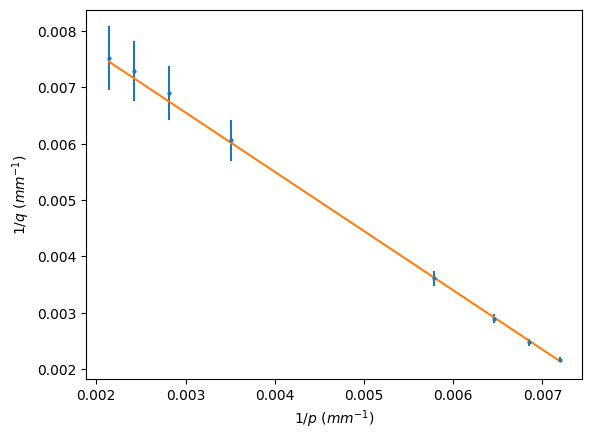
\includegraphics[width=0.6\textwidth]{immagini/100mm.png}
    \caption{Interpolazione lineare tra $\frac{1}{p}$ e $\frac{1}{q}$}
    \label{fig:3}
\end{figure}
Il test di adattamento del $\chi^2$ indica un adattamento del modello lineare del 99\%.
Il t-test restituisce t=0.86, associato a una compatibilità del 50,4\% con la distanza focale indicata sulla lente.
Sono poi stati raccolti i dati sugli ingrandimenti per quattro distanze sorgente schermo, che vengono riportati nella tabella sottostante. 

\begin{table}[htbp]
\centering
\begin{tabular}{c|cc|cc}
\hline
\hline
\textbf{Distanza} & \multicolumn{2}{c|}{\textbf{Misura 1}} & \multicolumn{2}{c}{\textbf{Misura 2}} \\
(\unit{mm}) & $M_{\text{sperimentale}}$ & $M_{\text{teorico}}$ & $M_{\text{sperimentale}}$ & $M_{\text{teorico}}$ \\
\hline
600 & \qty{3.650 \pm 0.095}{} & \qty{3.317 \pm 0.249}{} & \qty{0.325 \pm 0.026}{} & \qty{0.285 \pm 0.022}{} \\
550 & \qty{3.000 \pm 0.079}{} & \qty{2.767 \pm 0.202}{} & \qty{0.375 \pm 0.027}{} & \qty{0.332 \pm 0.026}{} \\
500 & \qty{2.450 \pm 0.066}{} & \qty{2.226 \pm 0.157}{} & \qty{0.475 \pm 0.028}{} & \qty{0.408 \pm 0.030}{} \\
450 & \qty{1.700 \pm 0.049}{} & \qty{1.601 \pm 0.109}{} & \qty{0.650 \pm 0.030}{} & \qty{0.579 \pm 0.041}{} \\
\hline
\hline
\end{tabular}
\caption{Confronto tra ingrandimento sperimentale e teorico al variare della distanza.}
\label{tab:ingrandimenti-2}
\end{table}

Come in precedenza, è stato effettuato un t-test di Student per verificare la compatibilità tra dati sperimentali e teorici, ottenendo per ciascuna coppia di valori t<2.

La distanza minima osservata è pari a \qty{405 \pm 5}{mm}, compatibile con quella teorica di \qty{400}{mm}.
\newpage